
\section{dHvA torque oscillation}

\subsection{Theory}

\begin{equation}
A(B,\phi,\theta,T)=A_0R_{\Gamma}R_TR_DR_{\textrm{mos}}R_{\textrm{dop}}R_sR_{\textrm{warp}}
\label{Eqn:2:OscilllationAmp}
\end{equation}

\begin{align}
R_T(B, \theta, T) &= \frac{X}/{\sinh{X}} \\
X                 &= \frac{2\pi^2k_Bm^*_{\textrm{therm}}T}{e\hbar B\cos{\theta}} \\
\label{Eqn:2:TempTermOscillationAmp}
\end{align}

\subsection{Mapping the Fermi surface}

\subsubsection{Background removal}
% TODO: Removal of background should not be done against 1/B as a rule.
% Include investigation as to low frequency peak
Previous standard practice was to remove a background polynomial fitted to the field or inverse field from the raw data before taking the FFT. \Fig\ref{Fig:2:BackgroundSubtraction} shows raw torque data taken over a range of angles\footnote{See section\ref{Sec:3:AngleDependentMeasurements} for full details} and a strong $H^2$ component can be observed as a result of the $R_{\Gamma}$ term in equation\ref{}. Subtracting a second order polynomial fitted to the \textit{inverse} field leaves a large artificial angle-dependant oscillation in $1\H$ in the residual which may be misconstrued as a signal from a low frequency Fermi surface orbit. For this reason it is recommended to subtract a second order polynomial fitted to field rather than inverse field for torque measurements.
\begin{figure}[h!]
    \begin{center}
        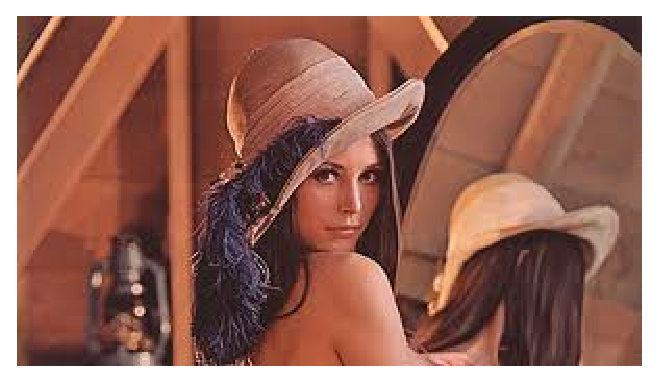
\includegraphics[scale=0.7]{Misc/TODO}
        \caption{Left panel shows the angle dependance of the raw torque signal  clearly showing a positive $H^2$ component for $\theta>0$ and a $-H^2$ component for $\theta<0$. Centre panel shows the FFT vs. angle for data with the 2nd order polynomial fitted to $1/H$ removed. A strong angle dependant peak at low frequency is seen. Right panel shows the same data but with a second order polynomial fitted to $H$ removed.}
        \label{Fig:2:BackgroundSubstraction}
    \end{center}
\end{figure}



\subsection{Measuring the spin mass}

\subsection{Measuring the band mass}

\subsubsection{Basic LK formula fitting}

Of all the damping terms in the \LK equation, only $R_T$ has any kind of temperature dependancy. This term also features the effective mass. By measuring oscillations at a fixed angle but with varying temperatures, the effective mass can be determined. However there is a difficulty in that in-order to observe oscillations, it is necessary to sweep the magnetic field, and many other damping terms have a field dependancy. To the first approximation, an inversely averaged applied field can be used in the \LK equation provided that the field sweep range is small. However there are a couple of techniques that were employed in order to overcome this shortcoming.

\subsubsection{Retrofitting ansatz LK formulae}
\label{Sec:2:LKRetrofitting}

One of the primary field-dependant contributions to the oscillation amplitude is the Dingle term scattering (equation \ref{Eqn:2:DingleTermOscillationAmp}). This has an exponential dependance with temperature. The Dingle factor, $\alpha$, can be determined by fitting a simplified version of equation \ref{Eqn:2:OscillationAmp} to oscillations which have been filtered to reduce the number of fitting parameters. Once we have the Dingle term, a series of ansatz data TODO...




\subsubsection{`Microfitting' the LK formula}
\label{Sec:2:LKMicrofitting}

\subsection{Method}

TODO: Angle correction

TODO: Temperature correction

\subsection{Yellow Magnet}

dHvA Measurements were all performed in Bristol on the `Yellow Magnet' system which was built by Oxford and can nominally operate up to \unit[20]{t} with use of the lambda plate although more typically is operated up to \unit[18]{T}. The sample sites on a one axis rotator and angle is determined by one of two orthogonal pick-up coils mounted on the sample stage weak, oscillating magnetic, field in

